\section{Sprungantwort Prozess}

\begin{figure}[h!]
	\centering
	\begin{subfigure}{0.475\textwidth}
		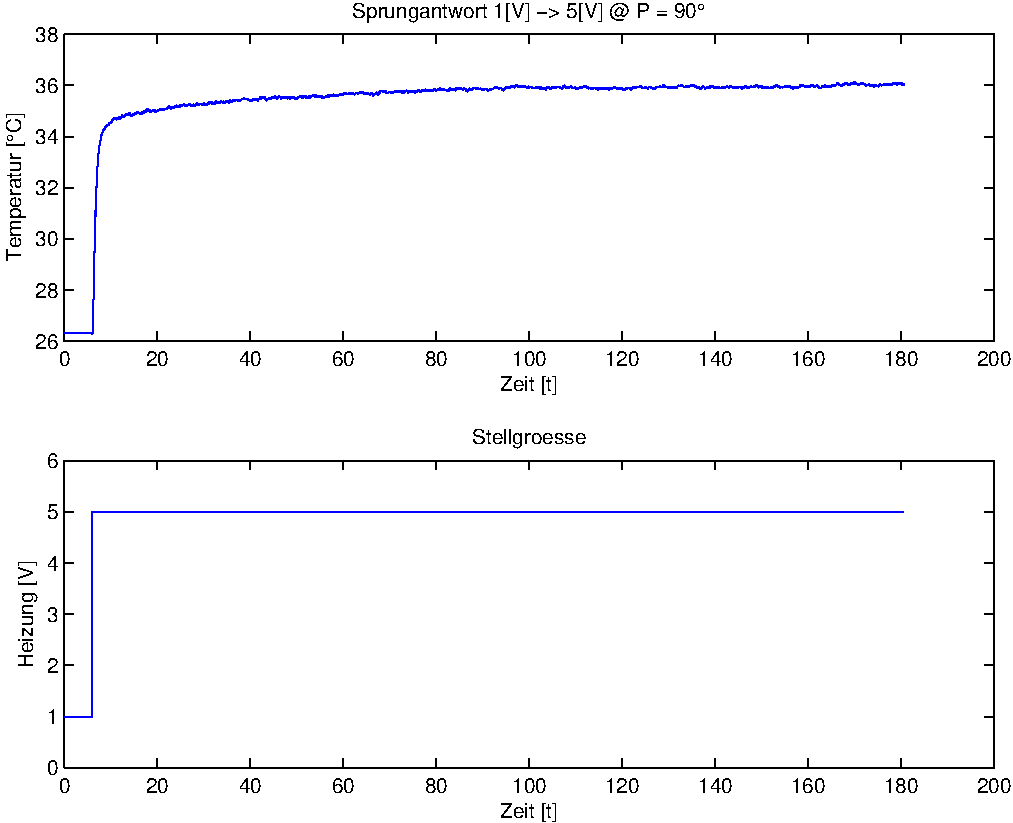
\includegraphics[width=1\textwidth]{03/step_full.pdf}
		\caption{Gesamter Verlauf}
	\end{subfigure}
	\hfill{}
	\begin{subfigure}{0.475\textwidth}
		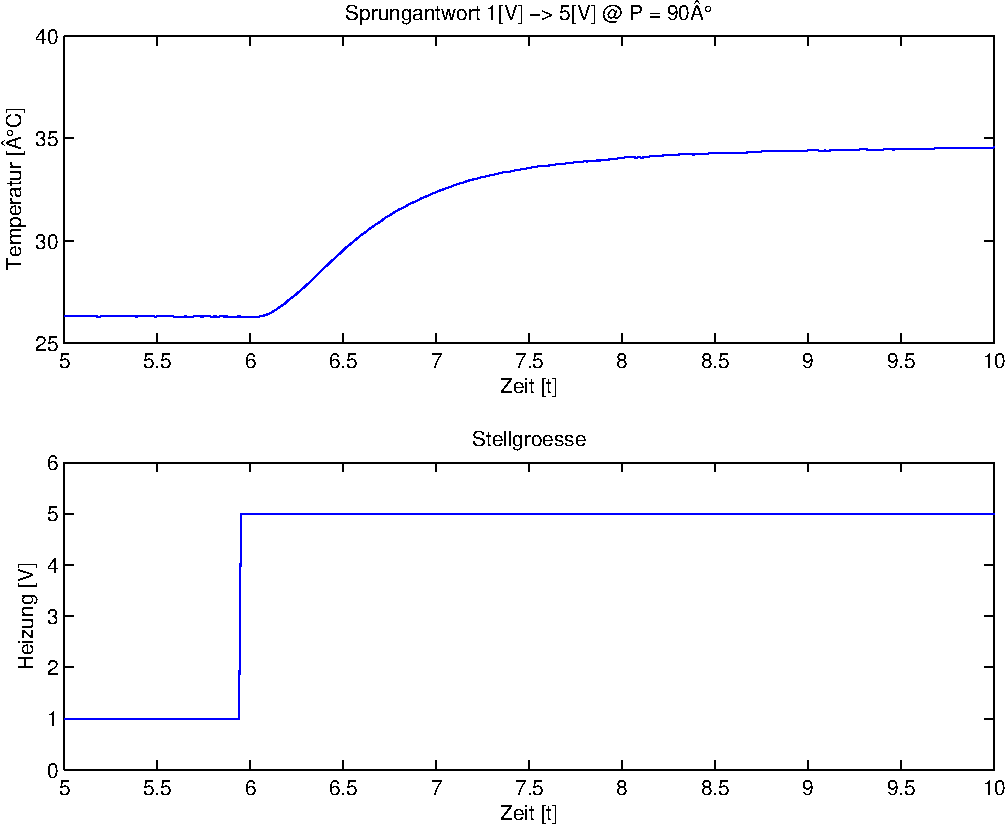
\includegraphics[width=1\textwidth]{03/step_full_scale.pdf}
		\caption{Skaliert auf Sprung}
	\end{subfigure}
	\caption{Sprungantworten des Prozesses bei Ventilstellung 90$^\circ$}
	\label{fig:03a}
\end{figure}

\begin{figure}[h!]
	\begin{subfigure}{0.475\textwidth}
		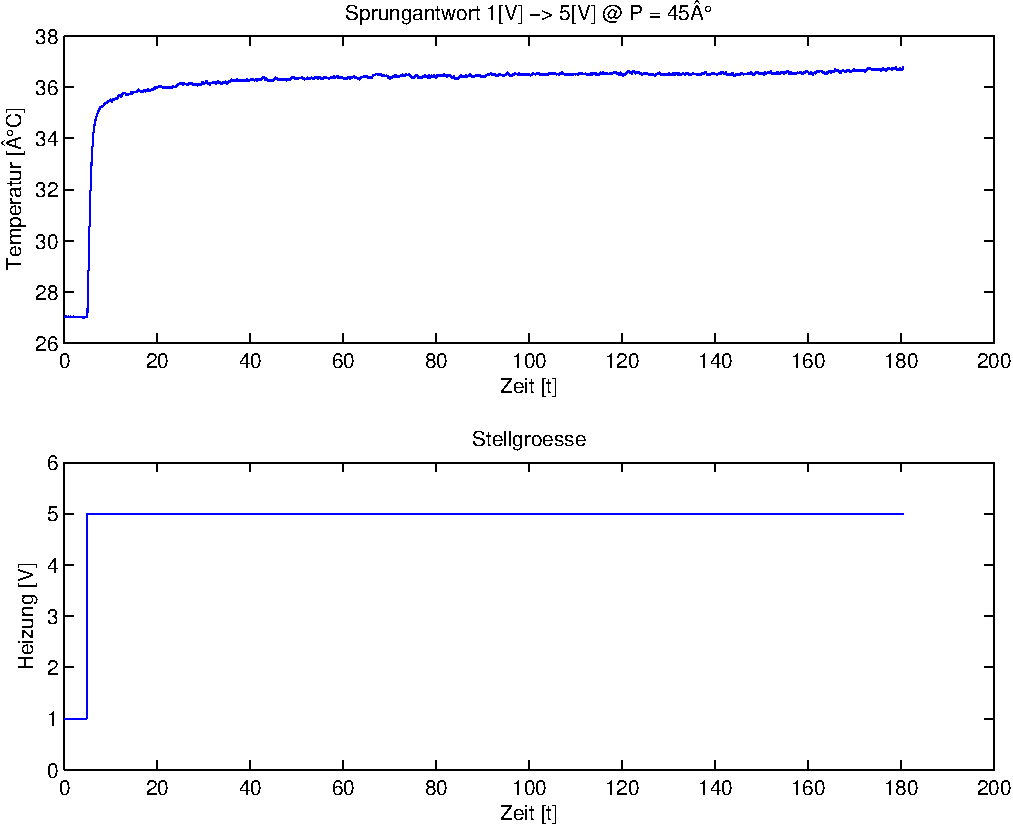
\includegraphics[width=1\textwidth]{03/step_half.pdf}
		\caption{Gesamter Verlauf}
	\end{subfigure}
	\hfill{}
	\begin{subfigure}{0.475\textwidth}
		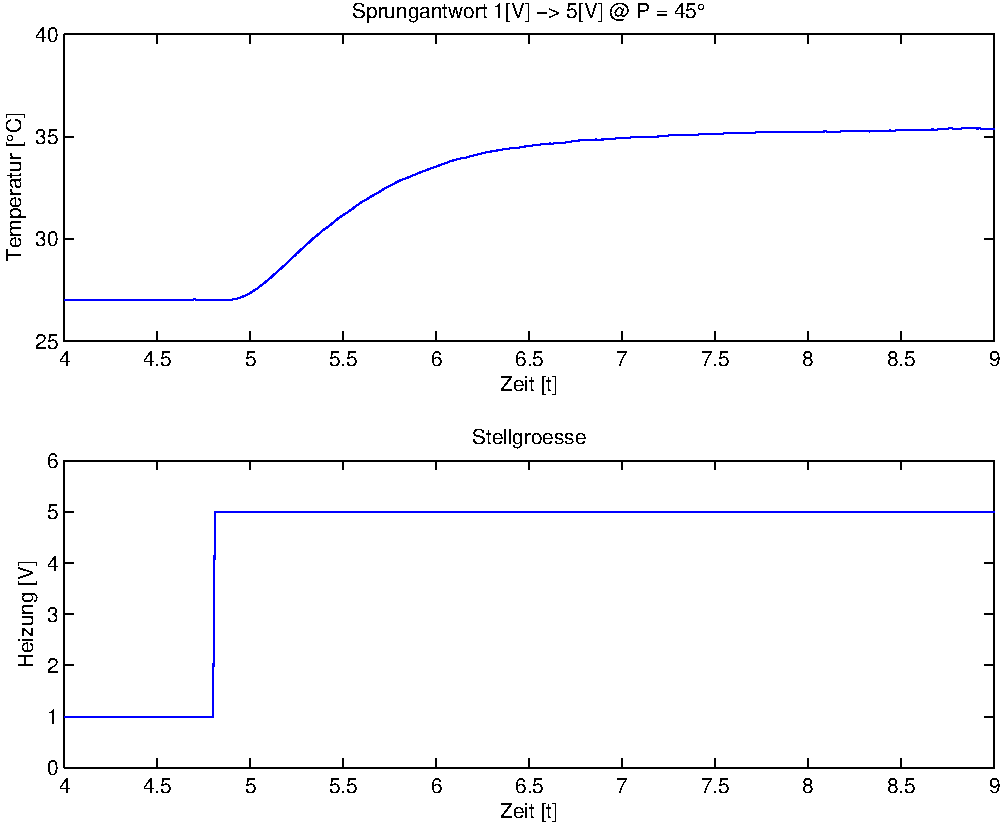
\includegraphics[width=1\textwidth]{03/step_half_scale.pdf}
		\caption{Skaliert auf Sprung}
	\end{subfigure}
	\caption{Sprungantworten des Prozesses bei Ventilstellung 45$^\circ$}
	\label{fig:03b}
\end{figure}
